\subsection{The Well}
{{\footnotesize
\noindent A 15 TB collection of ML-ready physics simulation datasets (HDF5), covering 16 domains-from biology to astrophysical magnetohydrodynamic simulations-with unified API and metadata. Ideal for training surrogate and foundation models on scientific data. 


\begin{description}[labelwidth=4cm, labelsep=1em, leftmargin=4cm, itemsep=0.1em, parsep=0em]
  \item[date:] 2024-12-03
  \item[version:] v1.0
  \item[last\_updated:] 2025-06
  \item[expired:] unknown
  \item[valid:] yes
  \item[valid\_date:] 2024-12-03
  \item[url:] \href{https://polymathic-ai.org/the\_well/}{https://polymathic-ai.org/the\_well/}
  \item[doi:] unknown
  \item[domain:] biological systems, fluid dynamics, acoustic scattering, astrophysical MHD
  \item[focus:] Foundation model + surrogate dataset spanning 16 physical simulation domains
  \item[keywords:]
    - surrogate modeling
    - foundation model
    - physics simulations
    - spatiotemporal dynamics
  \item[licensing:] BSD 3-Clause License
  \item[task\_types:]
    - Supervised Learning
  \item[ai\_capability\_measured:]
    - Surrogate modeling
    - physics-based prediction
  \item[metrics:]
    - Dataset size
    - Domain breadth
  \item[models:]
    - FNO baselines
    - U-Net baselines
  \item[ml\_motif:]
    - Foundation model, Surrogate
  \item[type:] Dataset
  \item[ml\_task:]
    - Supervised Learning
  \item[solutions:] 1
  \item[notes:] Includes unified API and dataset metadata; see 2025 NeurIPS paper for full benchmark details. Size: 15 TB. 

  \item[contact.name:] Ruben Ohana
  \item[contact.email:] rohana@flatironinstitute.org
  \item[datasets.links.name:] 16 simulation datasets
  \item[datasets.links.url:] \href{HDF5) via PyPI/GitHub}{HDF5) via PyPI/GitHub}
  \item[results.links.name:] ChatGPT LLM
  \item[fair.reproducible:] Yes
  \item[fair.benchmark\_ready:] Yes
  \item[id:] the\_well
  \item[Citations:] \cite{neurips2024_4f9a5acd}
\end{description}

{\bf Ratings:} ~ \\

\begin{tabular}{p{0.15\textwidth} p{0.07\textwidth} p{0.7\textwidth}}
\hline
Rating & Value & Reason \\
\hline
dataset & 5 & 15 TB of ML-ready HDF5 datasets across 16 physics domains. Public, well-structured,
richly annotated, and designed with FAIR principles in mind.
 \\
documentation & 4 & The GitHub repo and NeurIPS paper provide detailed guidance on dataset use,
structure, and training setup. Tutorials and walkthroughs could be expanded further.
 \\
metrics & 3 & Domain breadth and dataset size are emphasized. Standardized quantitative metrics for
model evaluation (e.g., RMSE, accuracy) are not uniformly applied across all domains.
 \\
reference\_solution & 3 & Includes FNO and U-Net baselines, but does not yet provide fully trained, reproducible
models or scripts across all datasets.
 \\
software & 5 & BSD-licensed software and unified API are available via GitHub and PyPI.
Supports loading and manipulating large HDF5 datasets across 16 domains.
 \\
specification & 4 & The benchmark includes clearly defined surrogate modeling tasks, data structure, and metadata.
However, constraints and formal task specs vary slightly across domains.
 \\
\hline
\end{tabular}

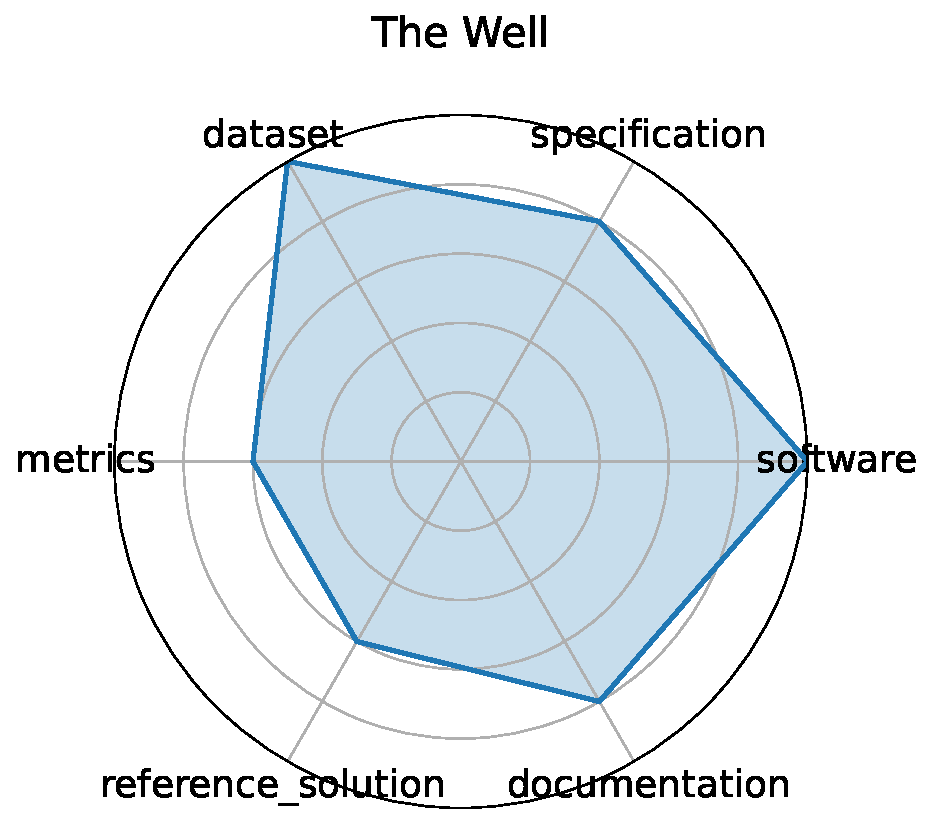
\includegraphics[width=0.2\textwidth]{the_well_radar.pdf}
}}
\clearpage